%%%%%%%%%%%%%%%%%%%%%%%%%%%%%%%%%%%%%%%%%
% Beamer Presentation
% LaTeX Template
% Version 1.0 (10/11/12)
%
% This template has been downloaded from:
% http://www.LaTeXTemplates.com
%
% License:
% CC BY-NC-SA 3.0 (http://creativecommons.org/licenses/by-nc-sa/3.0/)
%
%%%%%%%%%%%%%%%%%%%%%%%%%%%%%%%%%%%%%%%%%

%----------------------------------------------------------------------------------------
%	PACKAGES AND THEMES
%----------------------------------------------------------------------------------------
\documentclass{beamer}
% \usepackage{graphicx}
% \usepackage{caption}
% \usepackage{wrapfig}
% \usepackage{float}
% \usepackage{cmap}
% \usepackage{tikz}
% \usepackage{enumitem}
% \usepackage{multirow}
\usepackage{graphicx}
\usepackage{caption}
\usepackage{wrapfig}
\usepackage[utf8]{inputenc}
\usepackage[english, russian]{babel}

\mode<presentation> {

% The Beamer class comes with a number of default slide themes
% which change the colors and layouts of slides. Below this is a list
% of all the themes, uncomment each in turn to see what they look like.

%\usetheme{default}
%\usetheme{AnnArbor}
%\usetheme{Antibes}
%\usetheme{Bergen}
%\usetheme{Berkeley}
%\usetheme{Berlin}
%\usetheme{Boadilla}
%\usetheme{CambridgeUS}
%\usetheme{Copenhagen}
%\usetheme{Darmstadt}
%\usetheme{Dresden}
%\usetheme{Frankfurt}
%\usetheme{Goettingen}
%\usetheme{Hannover}
%\usetheme{Ilmenau}
%\usetheme{JuanLesPins}
%\usetheme{Luebeck}
\usetheme{Madrid}
%\usetheme{Malmoe}
%\usetheme{Marburg}
%\usetheme{Montpellier}
%\usetheme{PaloAlto}
%\usetheme{Pittsburgh}
%\usetheme{Rochester}
%\usetheme{Singapore}
%\usetheme{Szeged}
%\usetheme{Warsaw}

% As well as themes, the Beamer class has a number of color themes
% for any slide theme. Uncomment each of these in turn to see how it
% changes the colors of your current slide theme.

% \usecolortheme{albatross}
%\usecolortheme{beaver}
%\usecolortheme{beetle}
%\usecolortheme{crane}
%\usecolortheme{dolphin}
%\usecolortheme{dove}
%\usecolortheme{fly}
%\usecolortheme{lily}
%\usecolortheme{orchid}
%\usecolortheme{rose}
%\usecolortheme{seagull}
\usecolortheme{seahorse}
%\usecolortheme{whale}
%\usecolortheme{wolverine}

%\setbeamertemplate{footline} % To remove the footer line in all slides uncomment this line
%\setbeamertemplate{footline}[page number] % To replace the footer line in all slides with a simple slide count uncomment this line

%\setbeamertemplate{navigation symbols}{} % To remove the navigation symbols from the bottom of all slides uncomment this line
}

\usepackage{graphicx} % Allows including images
\usepackage{booktabs} % Allows the use of \toprule, \midrule and \bottomrule in tables

%----------------------------------------------------------------------------------------
%	TITLE PAGE
%----------------------------------------------------------------------------------------

\title[Закон Пашена]{Закон Пашена} % The short title appears at the bottom of every slide, the full title is only on the title page

\author{Грошев Максим Б01-206} % Your name
\institute[МФТИ] % Your institution as it will appear on the bottom of every slide, may be shorthand to save space
{
Московский физико-технический институт \\ % Your institution for the title page
% \medskip
% \textit{john@smith.com} % Your email address
}
\date{\today} % Date, can be changed to a custom date

\begin{document}

\begin{frame}
\titlepage % Print the title page as the first slide
\end{frame}

\begin{frame}
\frametitle{План} % Table of contents slide, comment this block out to remove it
\tableofcontents % Throughout your presentation, if you choose to use \section{} and \subsection{} commands, these will automatically be printed on this slide as an overview of your presentation
\end{frame}

%----------------------------------------------------------------------------------------
%	PRESENTATION SLIDES
%----------------------------------------------------------------------------------------

%------------------------------------------------
\section{Исторические сведения} % Sections can be created in order to organize your presentation into discrete blocks, all sections and subsections are automatically printed in the table of contents as an overview of the talk
%------------------------------------------------

% \subsection{Исторические сведения} % A subsection can be created just before a set of slides with a common theme to further break down your presentation into chunks

\begin{frame}
\frametitle{Исторические сведения}
\begin{wrapfigure}{left}{0.5\textwidth}
	\vspace{-15pt}
	\centering
	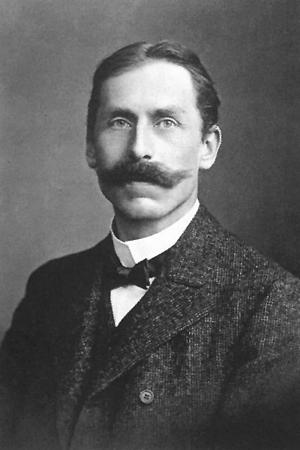
\includegraphics[width=0.3\textwidth]{ pics/pashen.jpg}
	\caption{Фридрих Пашен (1865-1947).}
\end{wrapfigure}

Немецкий физик, иностранный почетный член АН СССР (1930). Отметился трудами электрическим разрядам в
газах (установил закон, названный его именем, 1889), спектроскопии, спектральным и
измерительным приборам. Обнаружил спектральную серию водорода в инфракрасной области.
\end{frame}

%------------------------------------------------

\section{Закон Пашена}
\subsection{Формулировка закона}

\begin{frame}
\frametitle{Формулировка закона}

\textit{Разность потенциалов между электродами трубки, при которой начинается пробой газа, есть
функция произведения давления газа $P$ на расстояние между электродами $l$.}
\\~
\par
\textbf{Электрический пробой} - явление резкого возрастания тока в твёрдом, жидком или
газообразном диэлектрике (или полупроводнике) или воздухе, возникающее при приложении напряжения
выше критического.

\end{frame}

%------------------------------------------------


\begin{frame}
\subsection{Опыт Таунсенда}
\frametitle{Опыт Таунсенда}

\begin{wrapfigure}{left}{0.4\textwidth}
	\vspace{-35pt}
	\centering
	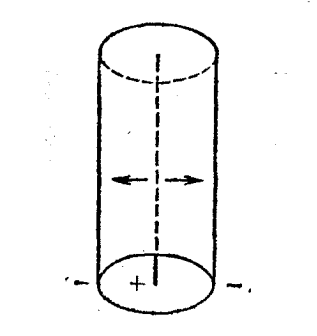
\includegraphics[width=0.3\textwidth]{ pics/setup.png}
	\caption{Установка опыта Таунсенда}
\end{wrapfigure}

$\alpha$ - среднее число ионов одного знака, производимое электроном на еденице пути длины
своего пути. Аналогичный смысл имеет имеет коэффициент $\beta $, характеризующий ионизирующую
способность положительных ионов. Причём  $\alpha > \beta$

\end{frame}

%------------------------------------------------

\begin{frame}
\frametitle{Опыт Таунсенда}

\begin{figure}[H]
        \centering
        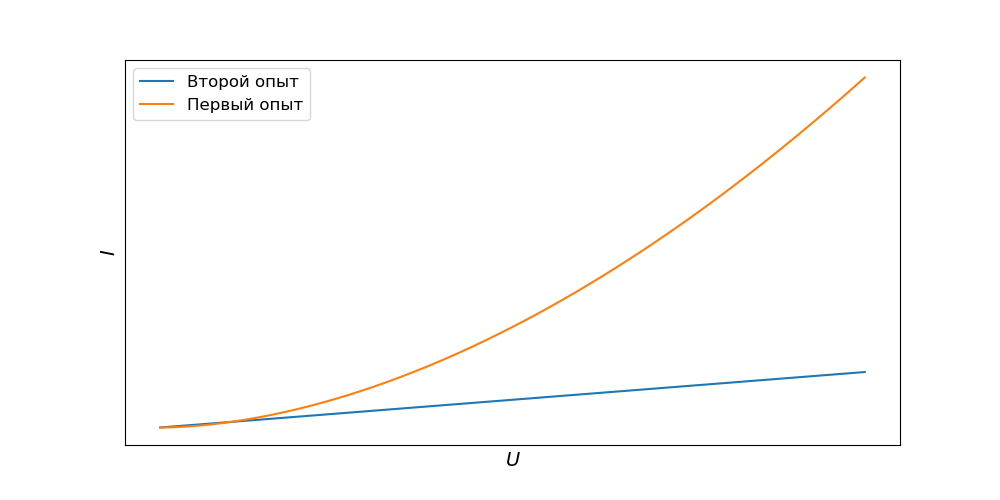
\includegraphics[scale=0.45]{./pics/taus.png}
        \caption{Результат опыта Таунсенда}
\end{figure}

\end{frame}

%------------------------------------------------

\begin{frame}
\subsection{Зависимость $\alpha$,  $\beta$ от $E$, $P$}
\frametitle{Зависимость $\alpha$,  $\beta$ от $E$, $P$}

\begin{itemize}
\item Условие ионизации
\begin{equation*}
    xE \geq U_{ion},
\end{equation*}
\item Число электронов, проходящих путь $x$ без столкновений
\begin{equation*}
    N = N_0\cdot e^{\frac{-x}{\overline l}}
\end{equation*}
\item Число ионизаций проводимых одним электроном
\begin{equation*}
    \alpha = \frac{1}{\overline l}\cdot e^{\frac{U_{ion}}{E \overline l}}
\end{equation*}
\end{itemize}

\begin{block}{Получаем зависимость}
\begin{equation*}
    \frac{\alpha}{P} = f(\frac{E}{P}),
\end{equation*}
\end{block}

\end{frame}

%------------------------------------------------

\begin{frame}
\subsection{Условие пробоя}
\frametitle{Условие пробоя}

\begin{itemize}
\item Условие пробоя
\begin{equation}
    (\beta + \gamma \cdot \alpha)e^{(\beta + \alpha)l} - (1 + \gamma)\alpha = 0
\end{equation}
\item Выражения для $\alpha$ и $\beta$
\begin{equation*}
    \alpha = P f (\frac{U}{lP})
\end{equation*}
\begin{equation*}
    \beta = P f_1 (\frac{U}{lP}),
\end{equation*}
\item Конечное выражение
\begin{equation*}
    F(\frac{U}{lP}) = 0,
\end{equation*}
\end{itemize}

\end{frame}

%------------------------------------------------

\begin{frame}
\frametitle{Важный результат}
\begin{block}{Полученный зависимость для напряжения пробоя}
\begin{equation*}
    U_{\text{пр}} = U_{\text{пр}}(lP),
\end{equation*}
\end{block}
\end{frame}

%------------------------------------------------
\begin{frame}

\frametitle{Характерные величины}

\begin{figure}[H]
        \centering
        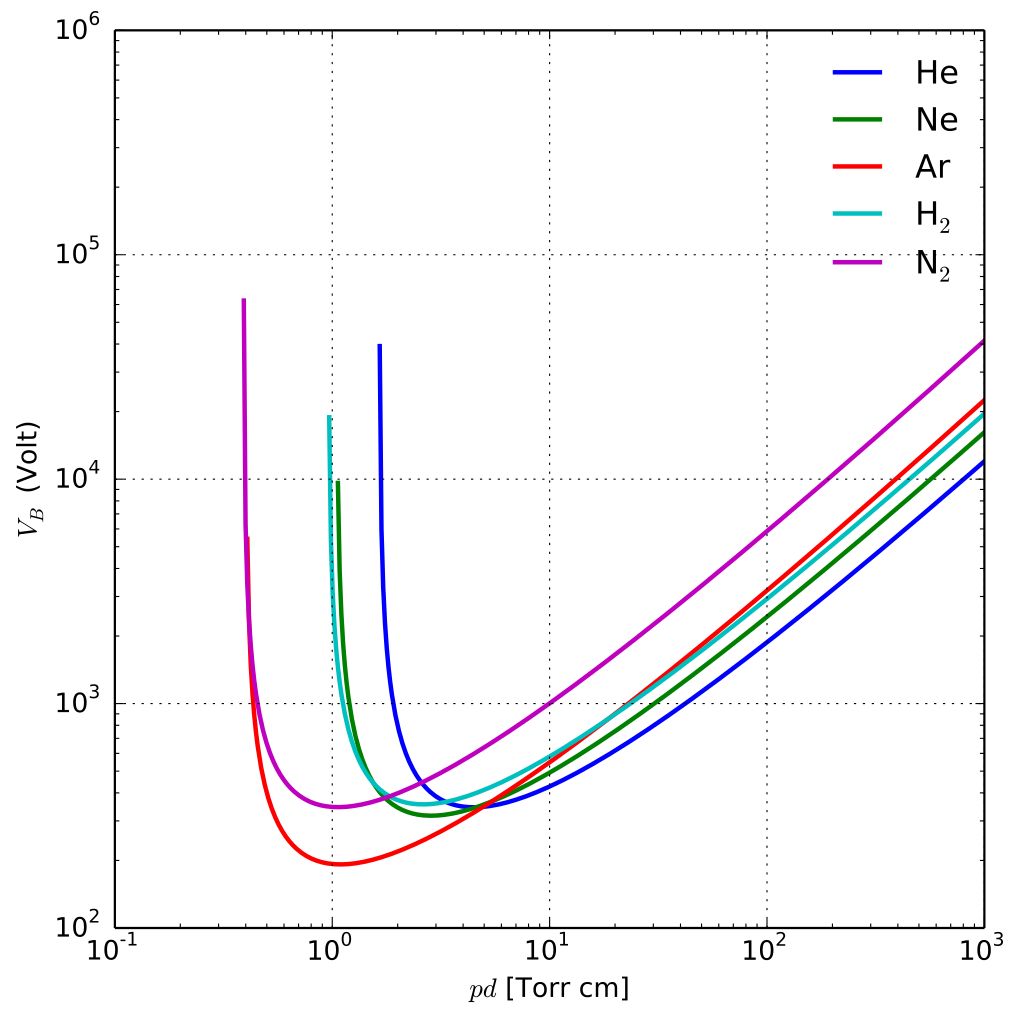
\includegraphics[scale=0.18]{./pics/pashean_lines.png}
        \caption{Эксперементальные данные Закона Пашена}
\end{figure}

\end{frame}

%------------------------------------------------

\section{Вывод}
\begin{frame}

\frametitle{Вывод:}
\vspace{-10pt}
\begin{block}{Полученный результат}
\begin{equation*}
    U_{\text{пр}} = U_{\text{пр}}(lP),
\end{equation*}
\end{block}
% \newline
% \\~
\par
Разность потенциалов между электродами трубки,
при которой начинается пробой газа, есть функция произведения
давления газа 8 на расстояние между электродами. Если в несколь
ких разрядных трубках с плоскими электродами создать условия,
при которых произведения $PL$ постоянны, то для всех трубок по
требуется одна и та же разность потенциалов, чтобы вызвать газо
вый разряд.

\end{frame}

%------------------------------------------------

\begin{frame}
\frametitle{Литература}
\footnotesize{
\begin{thebibliography}{99} % Beamer does not support BibTeX so references must be inserted manually as below
\bibitem[Smith, 2012]{p1} Д.В. Сивухин
\newblock
\newblock \emph{Общий курс физики $"$Электричество$"$}
\newblock \emph{Общий курс физики $"$Термодинамика$"$}

\end{thebibliography}
}
\end{frame}

%------------------------------------------------

\begin{frame}
\Huge{\centerline{Конец}}
\end{frame}

%----------------------------------------------------------------------------------------

\end{document}
